\documentclass[17pt]{extarticle}
%\usepackage[paperheight=4in]{geometry}
\usepackage[top=2cm, bottom=2cm]{geometry}
\pagestyle{empty} %no page numbering
\usepackage[utf8]{inputenc}
\usepackage{graphicx}
\usepackage{amsmath}
\usepackage{amssymb}
\usepackage{amsthm}
\usepackage{hyperref}

\newtheorem{theorem}{Theorem}
\newtheorem{proposition}[theorem]{Proposition}
\newtheorem{lemma}[theorem]{Lemma}
\newtheorem{example}[theorem]{Example}
\newtheorem{definition}[theorem]{Definition}
\newtheorem{remark}[theorem]{Remark}
\newtheorem*{theorem*}{Theorem}
\newtheorem*{condition*}{Condition}

\setlength\parindent{0pt} %no indent

\begin{document}
Throughout this section we will denote by $\alpha$ the shrinkage factor of line segments, by $\beta$ the angle between those later and by $L$ the initial segment's length. The limit set is denoted by $F$ and formally defined by
$$
F:=\{\lim_{n}\xi_n \ | \ \xi\in \mathcal{B}\}
$$
where $\mathcal{B}$ is the family of all branches starting at the root.
	
\begin{theorem} \label{cardinality}
	\textbf{Cardinality}\\
	The cardinality of the limit set $F$ is at most $2^{\omega}$ (continuity).
\end{theorem}
\begin{proof}
Each point in the limit is determined by at least one branch. Though in general several branches might share the same limit point. Thus the cardinality is not larger than that of all branches. The set $\{0,1\}^{\omega}$ of all ${0,1}$-sequences, which has cardinality $2^{\omega}$, can be naturally mapped bijective onto the set of branches - just interpret a $0$ of moving to the first child node and a $1$ to the second.
This shows altogether, the cardinality of all branches is $2^{\omega}$.
Since $\beta^{\omega}=2^{\omega}$ for any $\beta\in\omega$, a similar argument applies to trees with more than two child nodes as well.
\end{proof}

\begin{theorem}
	\textbf{Boundedness}\\
	The limit set always is bounded in $R^2$.
\end{theorem}
\begin{proof}
Consider a limit point $x$ and a branch $b=\{\xi_n \ | \ n\in\omega\}$ with $\lim_n \xi_n = x$. By triangle inequality we have
$$
|\xi_0 - \xi_n|\leq L\sum_i^n \alpha^i
$$
Here $|\cdot|$ denotes the Euclidean norm in $R^2$ and $\xi_0$ is the root of the tree.
On the one hand, by continuity of norm, we have $|\xi_0-\xi_n| \rightarrow |\xi_0-x|$. On the other hand the series on the r.h.s is converging against some $B\in\mathbb{R}$,
which shows
$$
|\xi_0 - x|\leq B
$$
Since $x$ has been chosen arbitrarily, this shows the entire limit set to be bounded.
\end{proof}

The last theorem shows together with the famous Heine-Borel theorem (\href{https://en.wikipedia.org/wiki/Heine\%E2\%80\%93Borel_theorem}{see here}), the limit set only can be discrete in case it is finite.

\begin{theorem} \label{unique_limits} 
	\textbf{Unique limits}\\
	Let $F$ result from a dual tree, that is one where each node has two child nodes.
	If we have the relation
	\begin{equation} \label{unique_branch_relation}
	\alpha<\frac{\sin(\beta/2)}{1+\sin(\beta/2)}
	\end{equation}
	then each branch has a unique limit.
	In this situation, the cardinality of $F$ is $2^{\omega}$.
\end{theorem}
\begin{proof}
	Let $x\in F$ and assume there are branches $(\xi_i)_i, (\eta_i)_i\in\mathcal{B}$ which both have $x$ as there limit. Because of the tree-structure, there must exist a maximal $n$ with $\xi_i=\eta_i$ for all $i\leq n$. This $n$ presents the level after which both branches starting being disjoint from each other. Up from this level both sub-branches (the left and right) are fully symmetric w.r.t the angle bisector. The idea is now to show that both branches cannot cross this bisector nor reach it in limit and hence cannot have the same limit as assumed. The following picture shall illustrate this situation:\\
	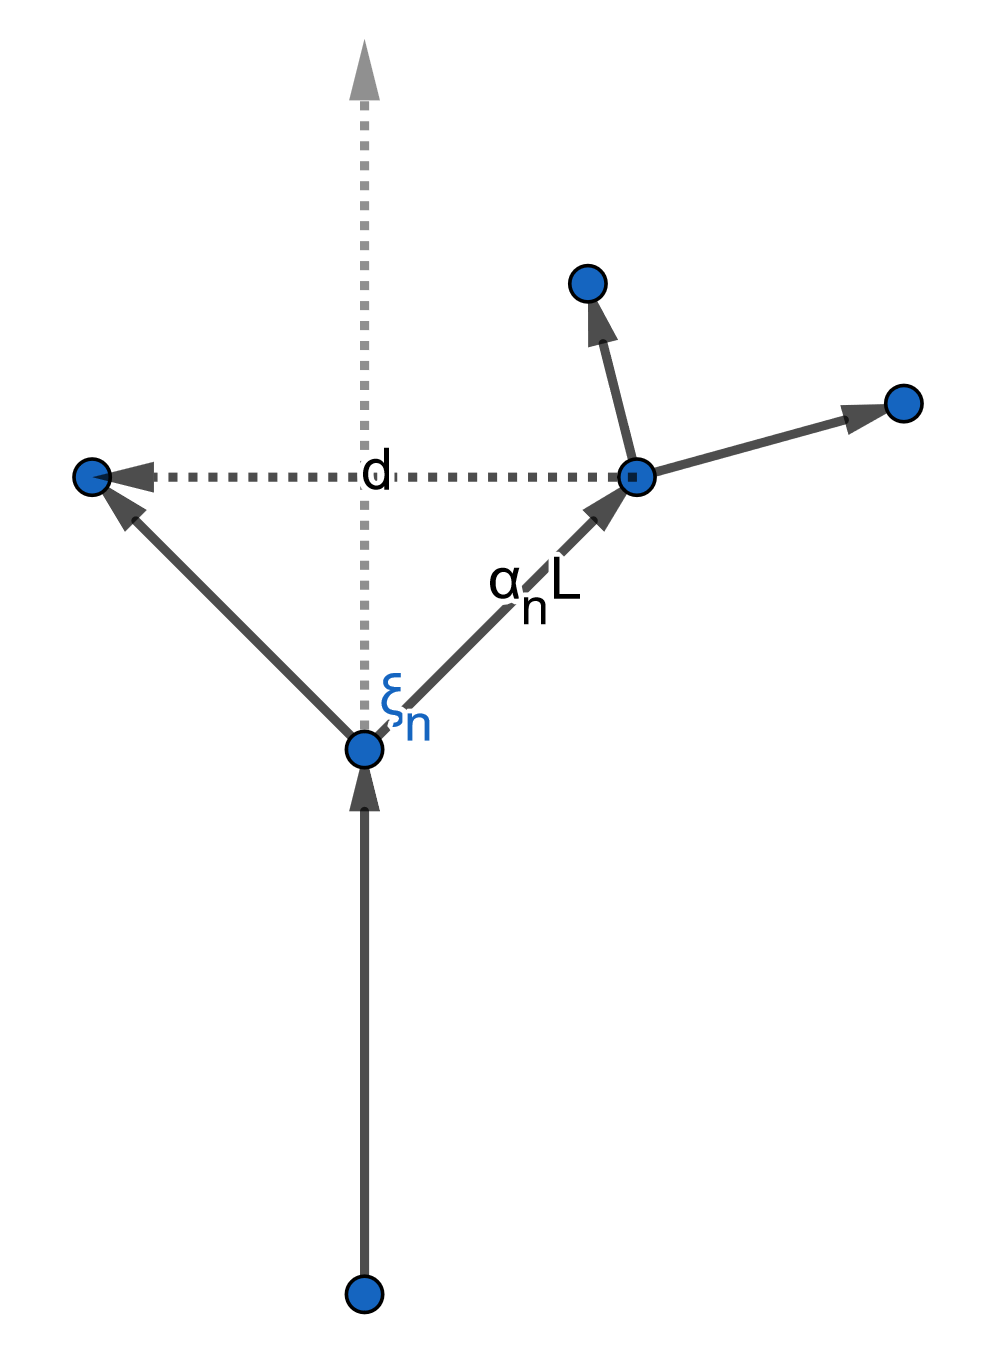
\includegraphics[width=10cm]{unique_branch}
	\\
	The distance $d/2$ is given by 
	$$
	\frac{d}{2}=\alpha^{n}L\sin\left(\frac{\beta}{2}\right)
	$$
	The two sub-trees, the one starting at the left node $\xi_{n+1}$ and the other starting at the right node $\eta_{n+1}$, produce limits which in worst case have distance 
	$$
	L\sum_{i\geq n+1}\alpha^i
	$$
	from  $\xi_{n+1}$ or $\eta_{n+1}$ correspondingly and along $d$. That is, the distance of such limits to the angle bisector is minimally 
	$$
	\frac{d}{2}-L\sum_{i\geq n+1}\alpha^i
	$$
	In order to finish the proof, we just have to show, that this difference is positive. We compute
	$$
	\sum_{i\geq n+1}\alpha^i=\alpha^{n+1}\sum_{i=0}\alpha^i=\alpha^{n+1}\frac{1}{1-\alpha}=
	\alpha^{n}\frac{\alpha}{1-\alpha}
	$$
	Using this and formula for $d/2$ we can formulate our targeted relation as
	$$
	\alpha^{n}\sin\left(\frac{\beta}{2}\right)>\alpha^n\frac{\alpha}{1-\alpha}
	$$
	which is equivalent to
	$$
	\sin\left(\frac{\beta}{2}\right)>\frac{\alpha}{1-\alpha}
	$$
	It is easy to see that this is equivalent with (\ref{unique_branch_relation}).\\
	The last statement is easily obtained by using the bijective relation between limit points and branches as stated in the proof of Theorem \ref{cardinality}.	
\end{proof}
So, under the prerequisites of preceding theorem, any $x\in F$ is in one to one correspondence with a branch. Similar results can be obtained for trees with more than two child nodes.

\begin{theorem}
	\textbf{Compactness}\\
	The limit set $F$ is closed and hence compact.
\end{theorem}
\begin{proof}
	The compactness follows from $F$ being bounded and closed. In order to show closeness let us consider any point $x\in\mathbb{R}^2$ which contains in each neighborhood a point from $F$. We will inductively construct a branch which has $x$ as limit and hence $x\in F$. The construction will be done for the case of a dual tree, but the more general case is done very similarly. Starting a the root one of both branches must have the property that it contains a sub-tree which has limit points arbitrary close to $x$. Repeating this selection on the next node and so on produces a branch $(\eta_n)_n$. Let us assume to the contrary that $x\neq\lim_n\eta_n$. Then there exists disjoint balls, $B_{\epsilon}(x)$ and $B_{\delta}(y)$, of $x$ resp. $y$. Now choose $M$ such that $\eta_n\in B_{\delta/2}(y)$ for all $n\geq M$ and moreover such that
	$$
	L\sum_{n>M}\alpha_n < \frac{\delta}{2}
	$$
	Such an $M$ exists since both, the sequence and series are Cauchy. The later condition actually tells that the sub-tree starting at $\eta_{M}$ entirely must lie within $B_{\delta}(y)$. But this is in contradiction with having constructed $(\eta_n)_n$ such that there exists a branch containing $\eta_M$ and having a limit in $B_{\epsilon}(x)$.
\end{proof}

\begin{theorem}
	\textbf{No isolated points}\\
	The limit-set $F$ has not isolated points.
\end{theorem}
\begin{proof}
	Let $x\in F$ and $U_{\epsilon}(x)$ be a neighborhood of $x$. Consider a branch $(\xi_n)_n$ which has $x$ as limit. We can find $M$ such that $\xi_M\in U_{\epsilon/2}$ and
	$$
	L\sum_{n>M}\alpha_n<\frac{\epsilon}{2}
	$$
	This implies that the sub-tree starting from $\xi_M$ entirely lies in $U_{\epsilon}$ and hence $U_{\epsilon}\cap F\neq\emptyset$, which completes the proof.
\end{proof}

\begin{theorem} \label{connectivity}
	\textbf{Connectivity}\\
	If (\ref{unique_branch_relation}) is met, then the limit set $F$ is hereditary disconnected.
\end{theorem}
\begin{proof}
	For ease of notation let us assume the tree is dual.
	Let $G\subset F$ be a subset consisting of at least two points. In order to show that $G$ is disconnected, we construct two open and disjoint sets $U, \ V$ such that $G\subset U\cup V$. For this, choose two points $x, \ y\in G$ and the maximum level $N$ for which their approaching branches have common nodes. Starting at the root, we construct along these common nodes two finite sequences of open sets. Let $\xi_n$ be any of these nodes. Then as in Theorem \ref{unique_limits} the angular bisector can be used to split the sub-tree into two halves. This means, the bisector defines two hyperplanes which separate $F$ into two disjoint sets. Moreover each part is contained in the inner of corresponding hyperplane, which we denote by $V_n$ and $U_n$ respectively.\\ \\
	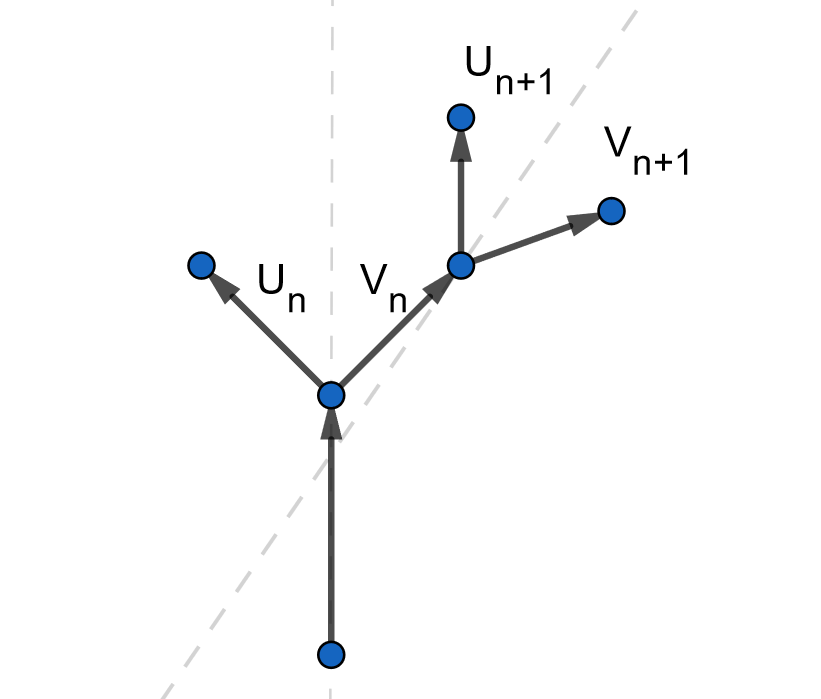
\includegraphics[width=10cm]{heredit_discon}
	\\
	The $V_n$'s are chosen such that all of the subsequent coming common nodes are contained inside: $\xi_{n+1}\in V_n$. At level $N$ we do yet another split of this type and ensure that the resulting open sets do contain $x$ resp. $y$. That is, $x\in V_N, \ y\in U_N$.
	We define $V:=V_1\cap\cdots\cap V_N$ and $U:=U_1\cup\cdots\cup U_N$. By construction these are disjoint open sets which cover all of $F$ and hence fulfill above requirements.\\	
	The argumentation for non-dual trees is similar.
\end{proof}

\begin{theorem}
	\textbf{Nowhere dense}\\
	If (\ref{unique_branch_relation}) is met, limit set $F$ is nowhere dense.	
\end{theorem}
\begin{proof}
	Since $F$ has already has been shown to be closed, we only need to verify that the interior is empty. Assume to the contrary it is not. There exists an open ball $B$ in $F$. This, as a subset of $F$, must be disconnected by Theorem \ref{connectivity}, which contradicts an open ball to be connected. So we have to drop the assumption.
\end{proof}

Altogether we have seen that under certain conditions the limit set of a fractal tree provides an example for a hereditary disconnected, compact, nowhere dense set without isolated points and with cardinality of the continuum.
\end{document}

	
